\chapter{Neural Ensemble Dynamics during Flexible Sensorimotor Behavior}
\label{NN_paper}

% Header
\fancyhead[R]{\small{ENSEMBLE DYNAMICS DURING FLEXIBLE BEHAVIOR}} %Running title

% Chapter Abstract
\lettrine[lines=3]{T}{he} ability to shift between repetitive and goal-directed actions is a hallmark of cognitive control. Previous studies have reported that adaptive shifts in behavior are accompanied by changes in neural activity in frontal cortex. However, neural and behavioral adaptations can occur at multiple time scales, and their relationship remains poorly defined. Here we developed an adaptive sensorimotor decision-making task for head-fixed mice, requiring them to shift flexibly between multiple auditory–motor mappings. Two-photon calcium imaging of secondary motor cortex (M2) revealed different ensemble activity states for each mapping. When adapting to a conditional mapping, transitions in ensemble activity were abrupt and occurred before the recovery of behavioral performance. By contrast, gradual and delayed transitions accompanied shifts toward repetitive responding. These results demonstrate distinct ensemble signatures associated with the initiation and termination of sensory-guided behavior and suggest that M2 leads the engagement of goal-directed response strategies that require sensorimotor associations.
\newpage

% Introduction
%\newpage
\nnsec{Introduction}

Operant behaviors are structured around stimuli, actions and outcomes. Successful execution of a task requires selecting actions that are consistent with the contingencies between these task variables. Control of action selection in the brain should be both stable and flexible. On the one hand, stability allows a subject to sustain high performance to maximize reward. On the other hand, flexibility is essential for quickly adjusting behavior when a change in contingencies occurs. Striking the delicate balance between stability and flexibility is therefore a key requirement of adaptive decision-making. Moreover, a lack of balance between these opposing aspects of cognitive control is a hallmark of psychiatric disorders \citep{griffiths2014translational}.

How do we know when to be stable or flexible in a changing environment? In tasks without explicit contextual cues, subjects may adjust their response strategy through reward feedback. Prior studies have observed task-dependent differences in neuronal firing rates and selectivity in multiple frontal cortical regions \citep{asaad2000task,rich2009rat,rodgers2014neural}. During periods of behavioral adjustment, evolution of cortical activity was found to be gradual and late, occurring on time courses that generally match or lag the improvement in task performance \citep{mitz1991learning,chen1995neuronal,pasupathy2005different,antzoulatos2011differences}. However, neurons in the frontal cortex exhibit substantial cell-to-cell variability in such time courses \citep{mitz1991learning}. Population activity may therefore be more useful for capturing circuit dynamics \citep{mante2013context,stokes2013dynamic,wills2005attractor}. Using ensemble recordings, two studies examined reward-guided adaptations, and they found the corresponding changes in network activity to be surprisingly abrupt \citep{durstewitz2010abrupt,karlsson2012network}. Determining the functional significance of these findings, however, will require quantitative comparisons of ensemble activity transitions that differ in their dynamics. Transitions that are relatively gradual versus abrupt, or that differ in onset with respect to behavioral changes, could reflect distinct underlying mechanisms for cognitive control.

To study adaptive sensorimotor decision-making in mice, we designed a head-fixed task that required animals to shift many times between three sets of stimulus–response contingencies. This task is a variant of arbitrary sensorimotor mapping, a classic model in which subjects are required to follow conditional rules \citep{bunge2005neural,white1999rule}, such as “for stimulus A, perform one action; for stimulus B, perform another action.” Once learned, the stimulus–response contingencies can then be switched, requiring the learning of novel mappings or retrieval of familiar associations. Associations are made by linking nonspatial stimuli or conditions to actions, and are therefore termed “arbitrary” \citep{wise2000arbitrary}. A number of brain regions are involved in arbitrary sensorimotor mapping, including the frontal lobe, striatum, hippocampus and thalamus \citep{wise2000arbitrary}. Within the frontal lobe, the dorsal premotor cortex has been implicated in the selection of motor programs based on antecedent conditions, as evidenced by the results of lesion studies \citep{petrides1985deficits,halsband1985premotor,nixon2004cortico}, electrophysiology \citep{mitz1991learning,chen1995neuronal}, functional imaging \citep{toni2001learning,boettiger2005frontal} and transcranial stimulation \citep{rushworth2002role} in humans and nonhuman primates.

Secondary motor cortex (M2) has been described as a potential rodent homolog of primate higher-order motor areas \citep{murray2000role,preuss1995rats}. Its location, adjacent to the medial prefrontal and primary motor regions, suggests that it may function as a cognitive–motor interface. A long line of research has linked the premotor cortex and neighboring regions to the generation of volitional movements \citep{nachev2008functional,schall2002monitoring,isoda2007switching}. Recent studies in rodents have also focused on the role of M2 in driving movements. Random-ratio lever-pressing was shown to become insensitive to reward devaluation in M2-lesioned mice, suggesting a role for M2 in goal-directed actions \citep{gremel2013premotor}. Neural activity is modulated before movement, reflecting involvement in action preparation and initiation \citep{sul2011role,erlich2011cortical,murakami2014neural}. Moreover, M2 neurons encode not only current action, but also prior choice and outcome, indicating a broader role in decision-making \citep{sul2011role}. One early study showed that rats with lesions of medial frontal cortex—a broader region that includes M2—had deficits in a visual conditional motor task \citep{passingham1988premotor}.

To elucidate the relationship between frontal ensemble activity and adaptive behavior, we used two-photon calcium imaging to record from M2 neurons in behaving mice. We found distinct population activity patterns associated with each of the three sets of stimulus–response contingencies. Moreover, following a contingency switch, transitions between ensemble patterns occurred earlier and were more abrupt when animals were required to abort repetitive actions and use a conditional rule. In fact, this change in ensemble activity state could be detected after only a few error trials, preceding the more gradual recovery of behavioral performance. Our results uncover distinct neural transitions associated with different phases of voluntary behavior and identify a leading role for M2 in engaging actions that require the use of sensorimotor associations.

% RESULTS
%\newpage
\section{Results}

\nnsub{Adaptive Decision-Making Task for Head-Fixed Mice}

We trained head-fixed mice to perform a task requiring flexible sensorimotor mapping. In each trial, fluid-restricted mice were presented with one of two randomized auditory stimuli, either logarithmic frequency-modulated sweeps from 5 to 15 kHz (`upsweep') or from 15 to 5 kHz (`downsweep'), and had to respond with a lick to the left or right port (FIGREF 1a). A correct response was rewarded with 2 \si{\uL} of water, while an incorrect response resulted in white noise. Trials were organized into blocks (Fig. 1b), each with a distinct set of stimulus--response contingencies: `sound-guided' (upsweep-left; downsweep-right), `action-left' (upsweep-left; downsweep-left), and `action-right' (upsweep-right; downsweep-right). When performance reached a criterion of 85\% correct over 20 trials, a new block began with different contingencies. Sound and action blocks alternated, and no contextual cue was given to signal the block transition. Therefore, performance beyond the first block required flexible response selection and outcome monitoring. Mice were prepared for this task by initial training to an expert level on two-choice auditory discrimination; i.e., $\sim 30$ d on a task with only sound-guided trials. Here, we present data from mice with fewer than 6 sessions of experience in the adaptive decision-making task.

\begin{figure}[htbp]

\begin{center}
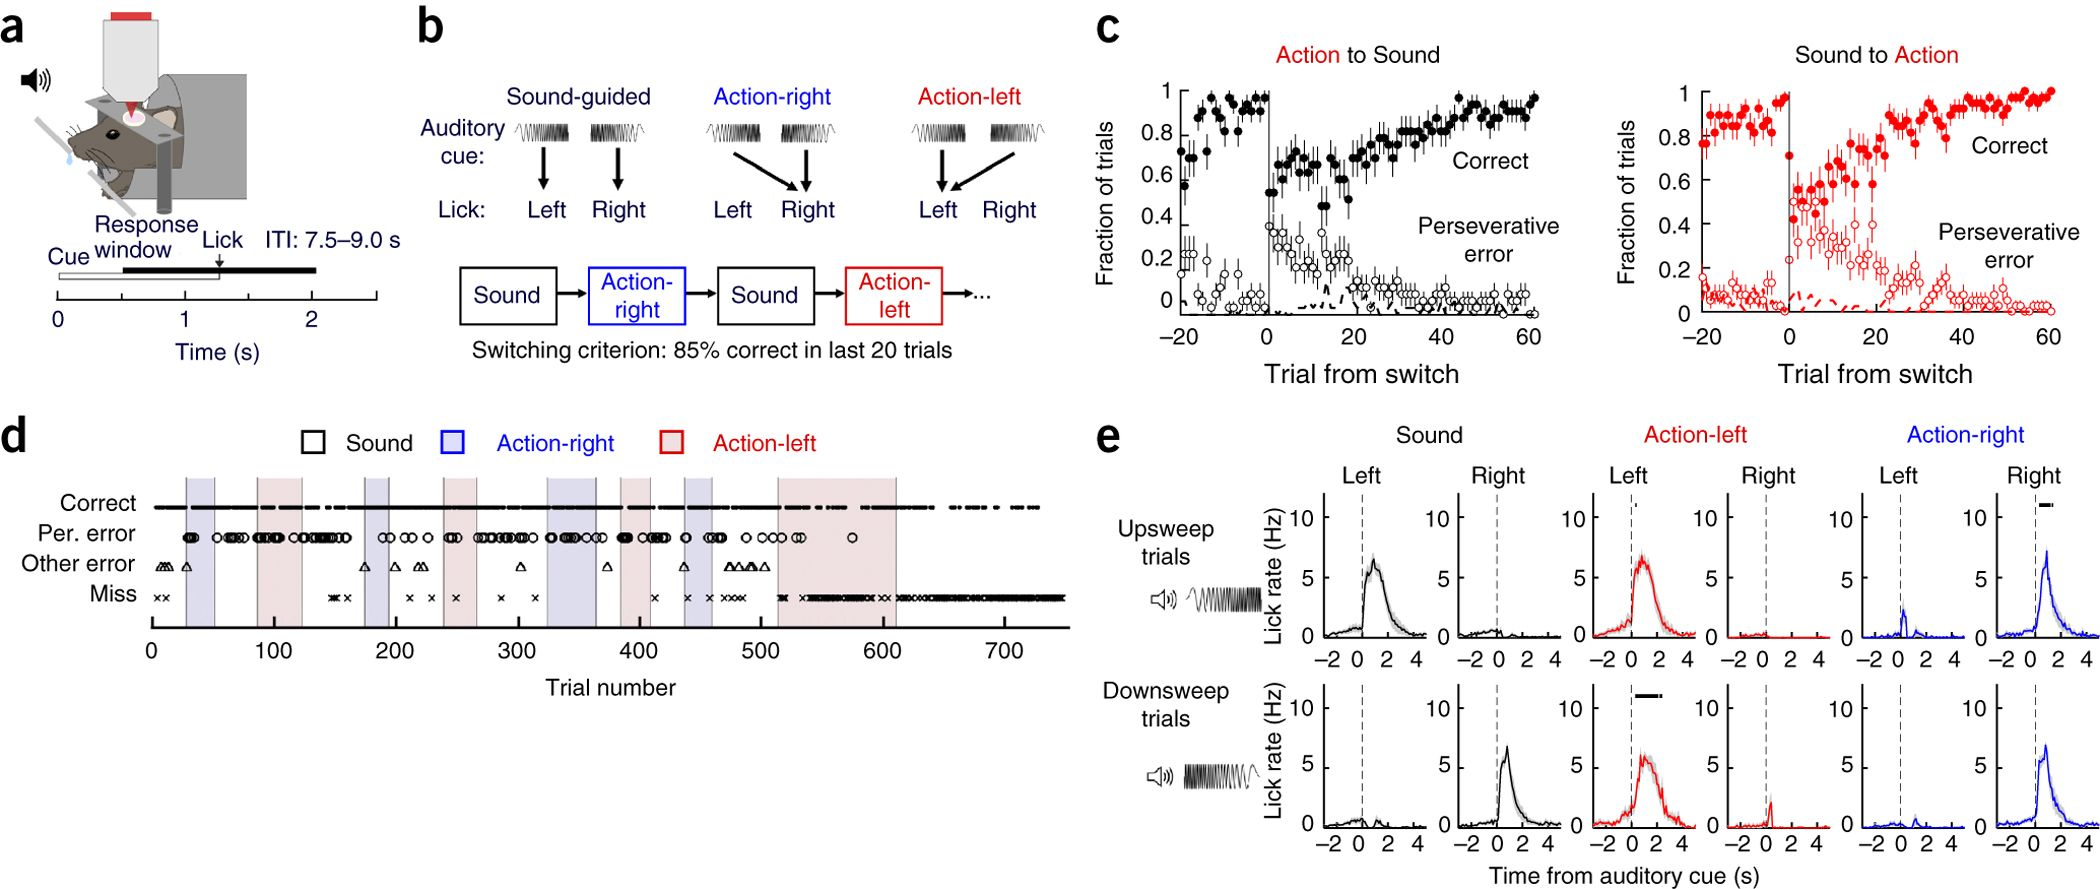
\includegraphics[width=\textwidth]{Figures/NN_fig1.jpg} 
\end{center}

\caption[Behavioral performance of head-fixed mice in an adaptive sensorimotor decision-making task]
{Behavioral performance of head-fixed mice in an adaptive sensorimotor decision-making task.
(A) Schematic of experiment. Each trial begins with an auditory cue. A response window starts 0.5 s after cue onset, during which the first lick is recorded as the response for that trial. Water reward is delivered contingent on a correct response. ITI, intertrial interval. (B) Schematic of stimulus–response mappings and block design. (C) Behavioral performance surrounding a block switch from action to sound (left) or sound to action (right). Filled circles, hit rate. Open circles, perseverative error rate. Dotted line, other error rate. $N=$ 33 action-to-sound switches and 38 sound-to-action switches. (D) Performance from one example behavioral session. Trial outcomes: correct (filled circles), perseverative error (open circles), other error (open triangles), or miss (cross). Vertical line, rule switch. (E) Left and right lick rates for upsweep or downsweep sound cues during all correct sound-guided (black), action-left (red) and action-right (blue) trials. For each choice direction, lick rates during action trials were compared to sound trials in 0.1 s bins; black bars, significant differences ($p < 0.01$, paired t-test). All data presented as $mean \pm SEM$. $N = 9$ sessions from 5 mice.}

\label{fig:NN_fig1}
\end{figure}

% \begin{FPfigure}

% \begin{center}
% 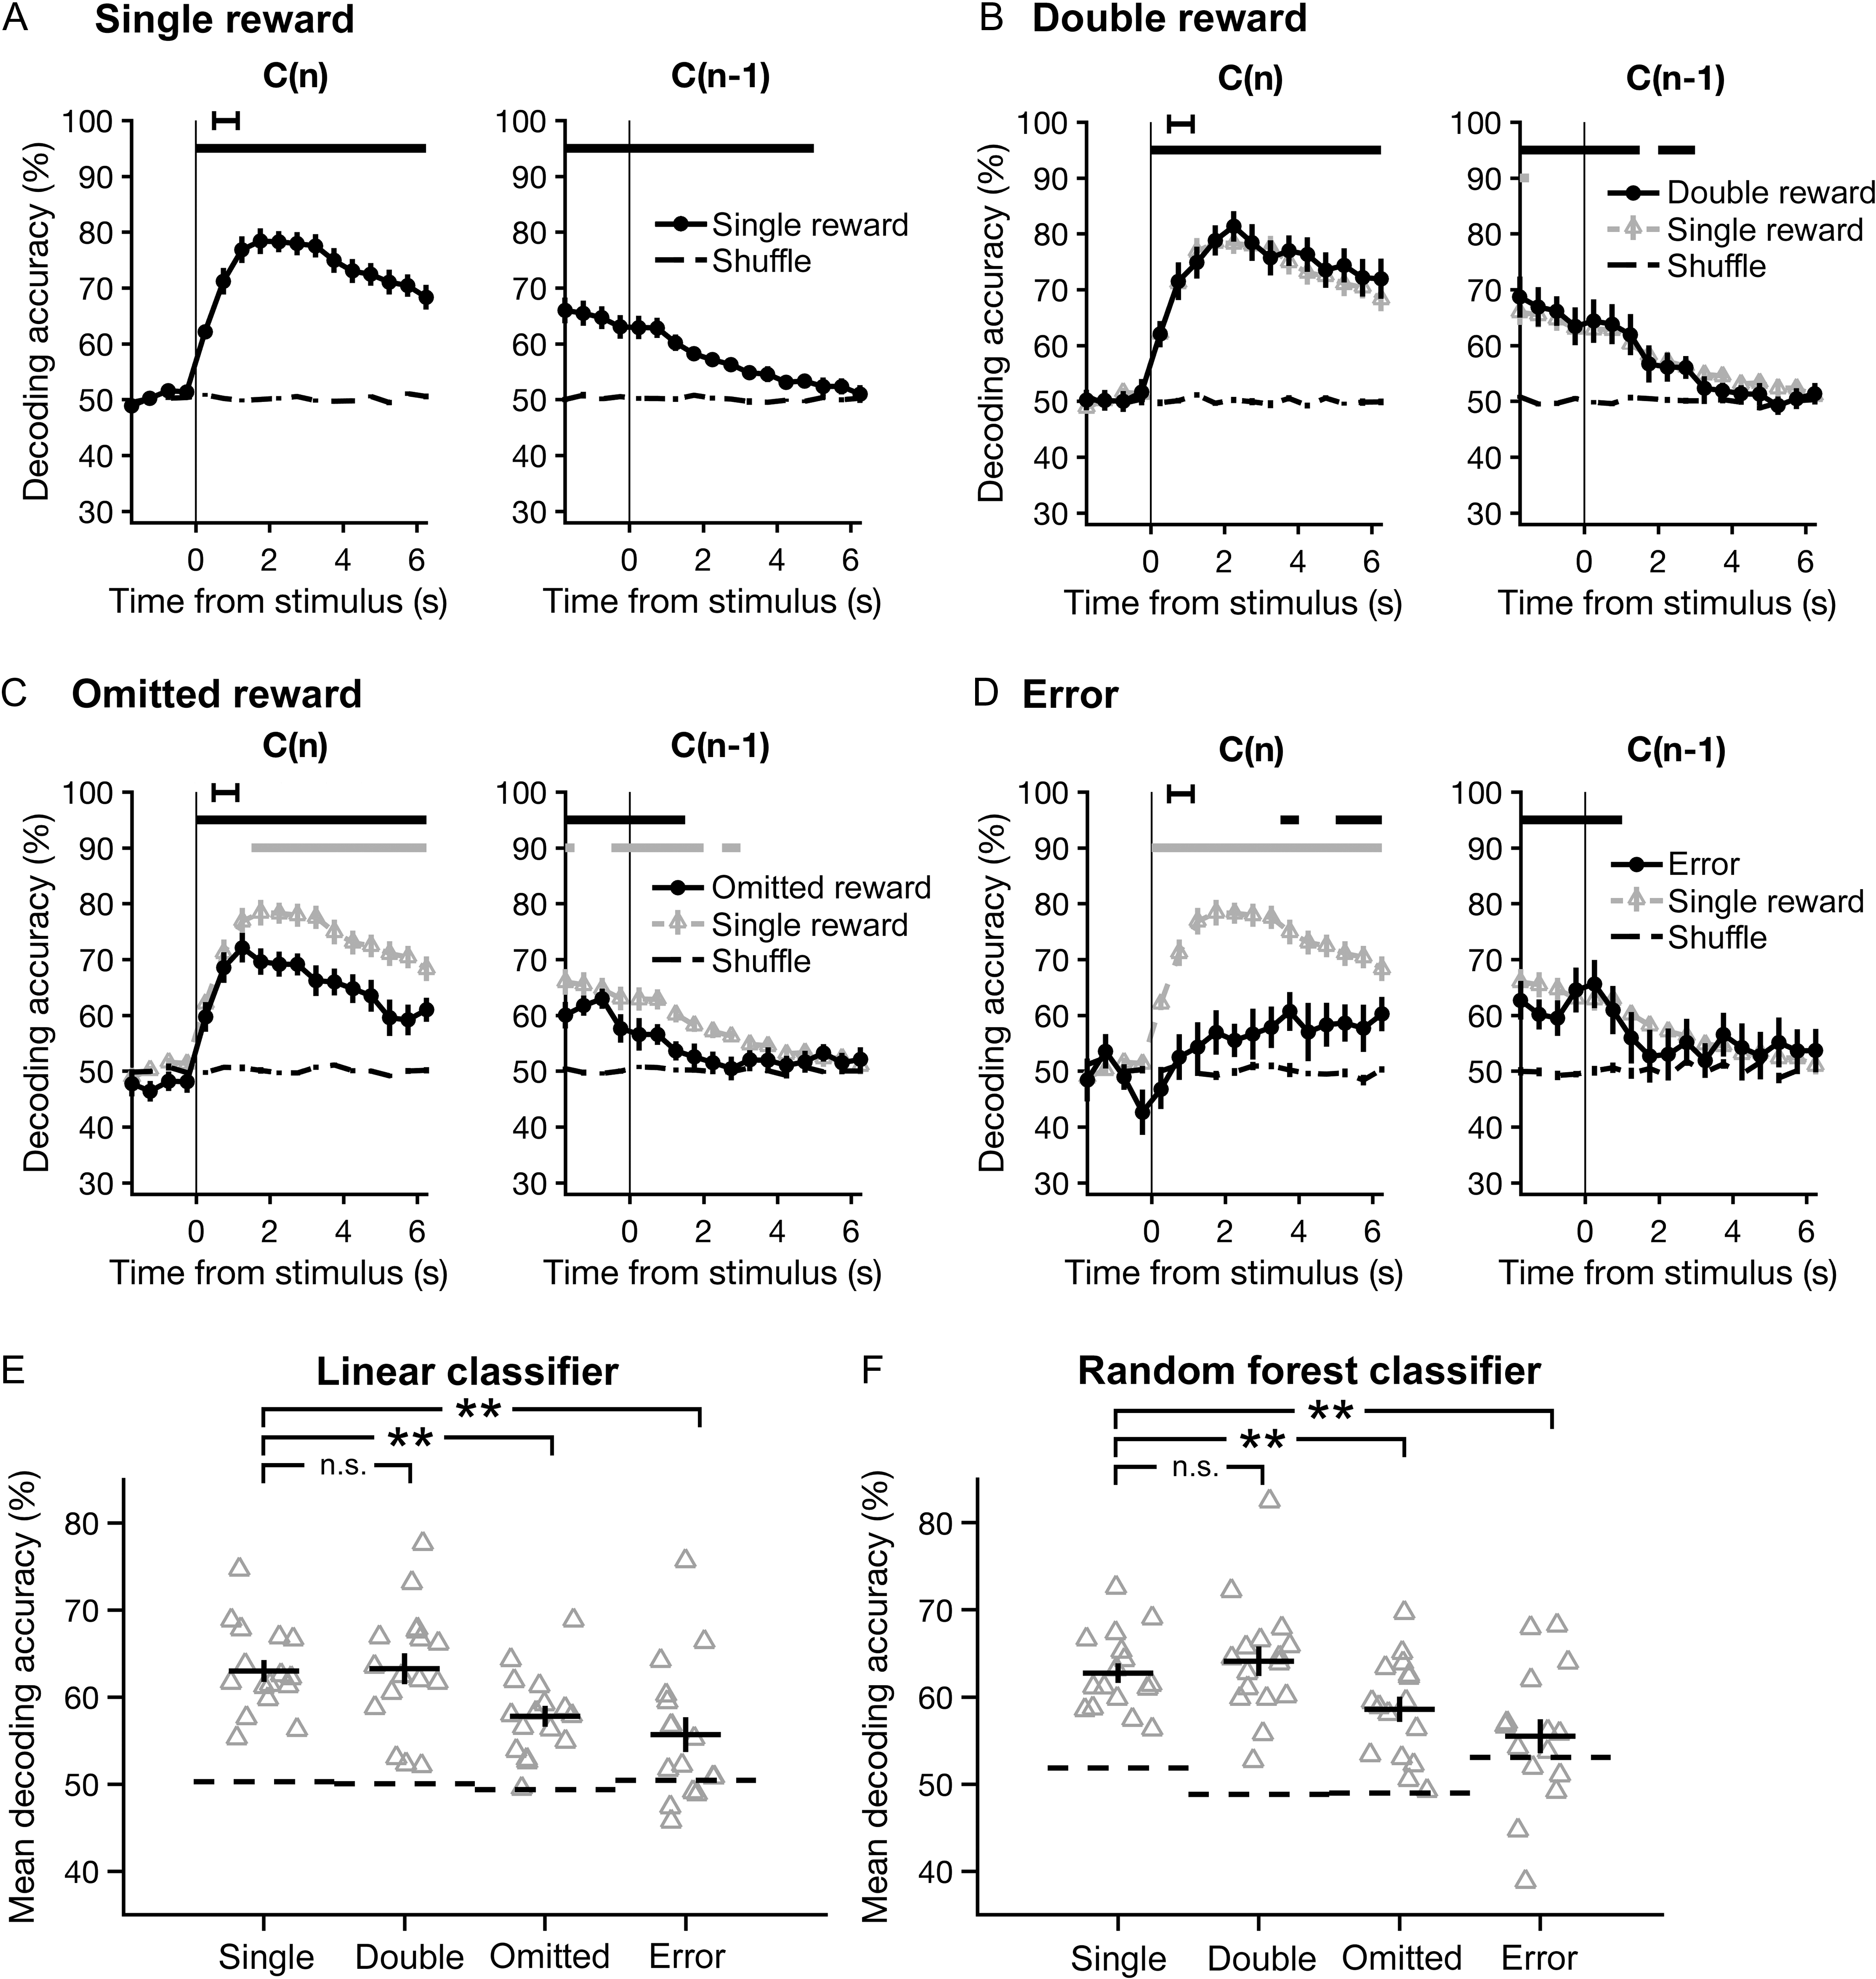
\includegraphics[width=\textwidth]{Figures/CC_fig6.png} 
% \end{center}
% \small{Figure \ref{fig:CC_fig6} Decoding accuracy diminished during omitted-reward and error trials. }

As expected, a switch in contingencies was associated with an immediate drop in correct response rate (FIGREF 1c,d). Most incorrect responses were perseverative errors, indicating a failure to update response strategy for $\sim 20$ trials after the switch. We obtained concurrent calcium imaging and behavioral data during 9 sessions from 5 mice (REF Table 1). On average, these mice performed $418 \pm 49$ trials per session, including $296 \pm 38$ rewarded trials and $9 \pm 1$ block switches ($mean \pm SEM$; range: 6–19 switches; REF Supplementary Fig. 1a). 

To quantify motor output, we calculated the mean lick rates and the time of first lick for different trial types. Overall, licks were tightly locked to the time of auditory cue during correct trials (REF Fig. 1e). For congruent trials (in which stimulus--response contingencies match), lick rates were indistinguishable across sound and action blocks. For incongruent trials (for example, left action for upsweep during sound block versus downsweep during action-left block), there was a noticeable difference in mean lick rates and an increased latency to first lick (REF Supplementary Fig. 2). Nevertheless, the major determinant for the shape of the lick distribution was response direction: i.e., whether the animal chose left or right (REF Fig. 1e). 

Additionally, we used video tracking to monitor whisker and hindpaw positions, and found that their movements also depended mostly on response direction (REF Supplementary Fig. 3). Therefore, although licks were the means for making operant responses in this head-fixed setup, mice performed more complex motor programs to indicate their choices.

\nnsub{Silencing M2 Selectively Impairs Shift to Sound-Guided Actions}
To determine whether frontal cortical activity is necessary for adaptive decision-making in our task, we used the GABA\textsubscript{A} receptor agonist muscimol to inactivate M2 bilaterally. Muscimol (5 mM, 46 nL per hemisphere) or saline vehicle was injected $\sim 1$ h before behavioral testing ($n = 11$ mice; REF Fig. 2a and Supplementary Table 1). We injected low-molecular-weight fluorescein to estimate the extent of the affected region, which included M2 and part of cingulate cortex (Cg1), but not other neighboring regions (REF Supplementary Fig. 4).
\begin{figure}[htbp]

\begin{center}
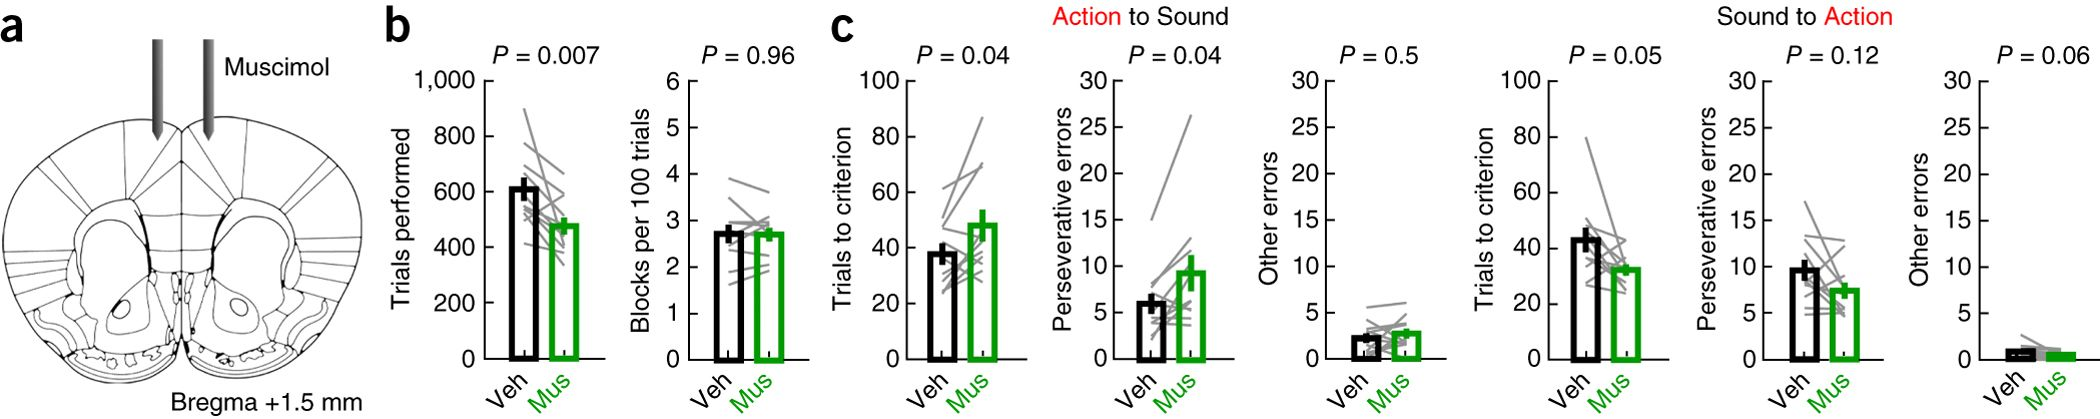
\includegraphics[width=\textwidth]{Figures/NN_fig2.jpg} 
\end{center}

\caption[Bilateral inactivation of M2 impairs adjustment to sound rule]
{Caption}

\label{fig:NN_fig2}
\end{figure}

Compared to controls, muscimol-injected mice performed fewer trials (Fig. 2b; saline: $608 \pm 42$, muscimol: $476 \pm 31$, $mean \pm SEM$; $p = 0.007$, $W = 62$, Wilcoxon signed-rank test), although there was no difference in the number of switches per 100 trials (saline: $2.7 \pm 0.2$, muscimol: $2.7 \pm 0.1$, $mean \pm SEM$; $p = 0.96$, $W = 34$). Inactivation had no effect on the timing or rates of lick motor output (REF Supplementary Fig. 5). 

Notably, separate analyses of sound and action blocks revealed selective impairments in the animals' ability to engage sound-guided actions, evidenced by a marked (55\%) increase in the number of perseverative errors per block (Fig. 2c; saline: $5.7 \pm 1.1$, muscimol: $8.9 \pm 1.9$, $mean \pm SEM$; $p = 0.042$, $W = 10$, Wilcoxon signed-rank test), and a greater number of trials to reach criterion (saline: $38 \pm 4$, muscimol: $48 \pm 6$, $mean \pm SEM$; $p = 0.042$, $W = 10$). Nevertheless, muscimol-injected mice eventually reached the criterion of $\ge 85\%$ correct, indicating that the transition to a high level of performance was slowed, but not blocked, by M2 inactivation. 

Silencing had the opposite effect on shifts into action blocks, during which the mice required fewer trials to reach criterion, although this effect fell short of statistical significance (saline: $43 \pm 4$, muscimol: $32 \pm 2$, $mean \pm SEM$; $p = 0.054$, $W = 55$). 

These results indicate a causal role for M2 in the flexible control of action selection. Additionally, the opposing effects of silencing are useful for understanding how the mouse performs the outlined task. One solution to the task would be to forget and relearn the relevant stimulus–response associations after each contingency change, as in a reversal task33. This approach predicts symmetric changes in behavior following perturbations. An alternative approach would be to rely on these associations for sound-guided trials and then ignore them during action blocks to favor repeated selection of the same response. In this case, the mouse would perform the task by shifting the balance between conditional and unconditional means of responding. The asymmetric deficits observed in our experiments are consistent with the second approach and implicate M2 in the breaking of repetitive actions and biasing choices based on learned associations.

\nnsub{Imaging Task-Related Activity at Cellular Resolution in M2}
To characterize neural activity in layer 2/3 of M2, we injected an adeno-associated virus encoding GCaMP6s (AAV1-Syn-GCaMP6s-WPRE-SV40; Fig. 3a). GCaMP6s is a genetically encoded calcium indicator that exhibits a $\sim 25\%$ rise in fluorescence intensity per action potential in cortical pyramidal neurons34. While mice performed the adaptive decision-making task, we used two-photon microscopy to record from $62 \pm 6$ cells per field of view ($mean \pm SEM$; range, 26–83 cells; $N = 9$ sessions from 5 mice; Fig. 3b). 
\begin{figure}[htbp]

\begin{center}
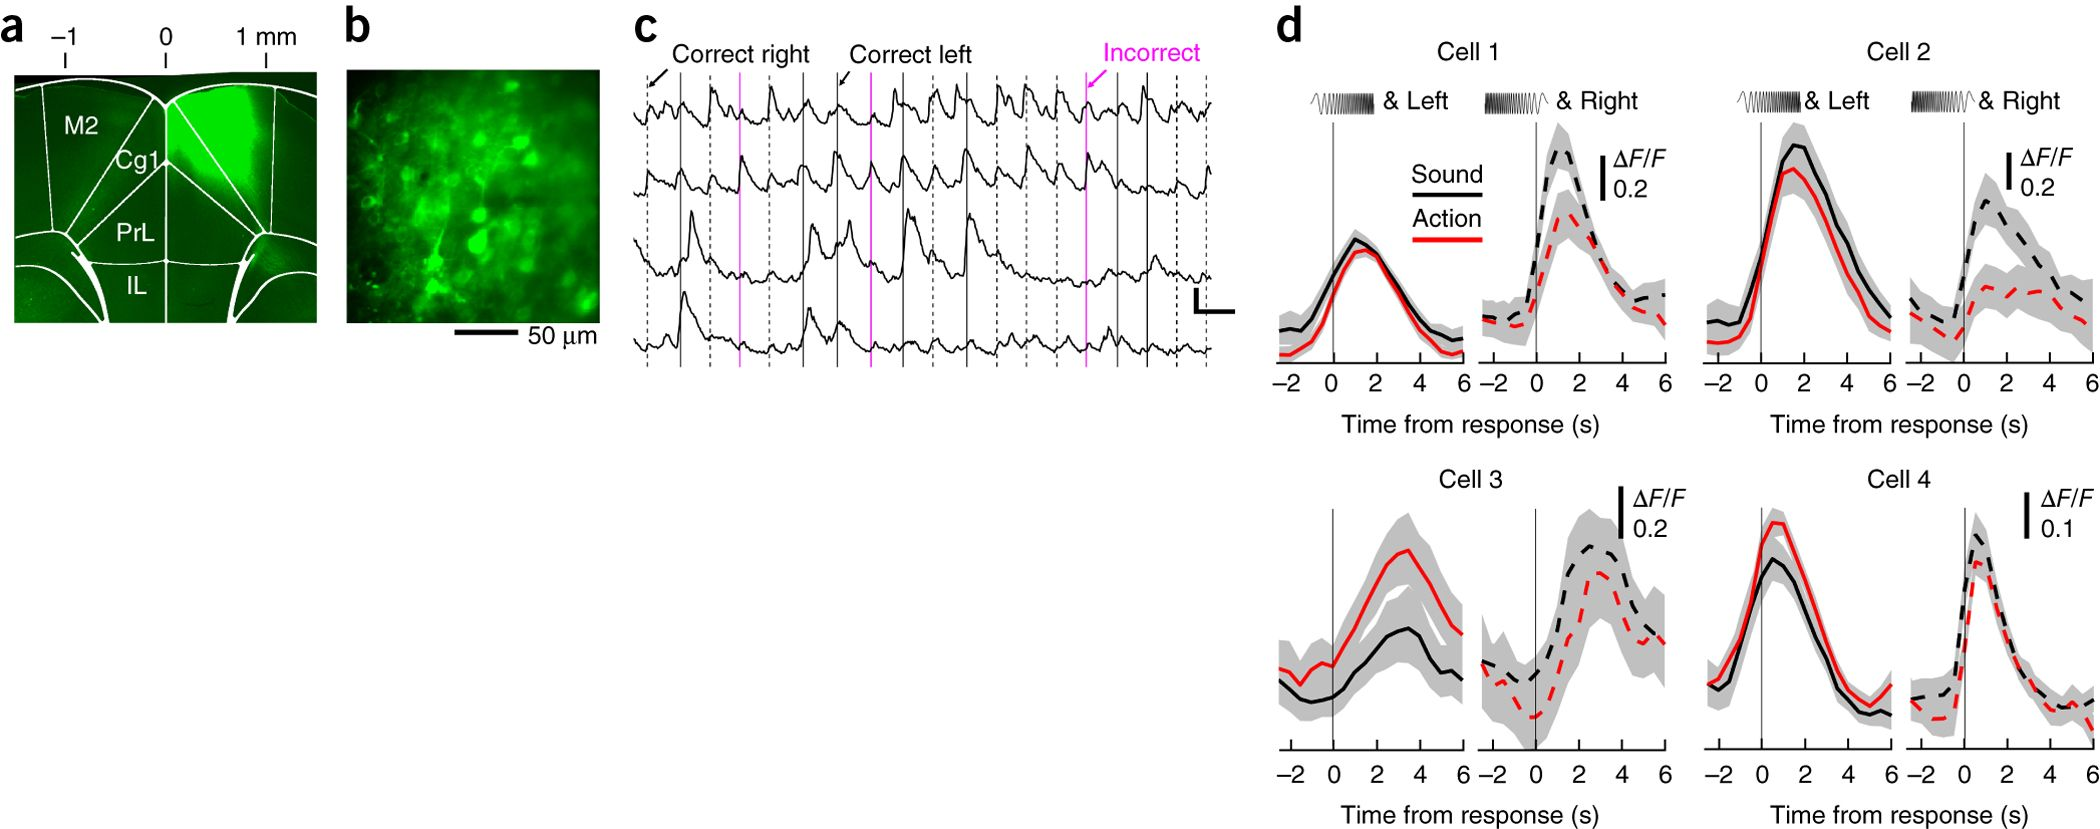
\includegraphics[width=\textwidth]{Figures/NN_fig3.jpg} 
\end{center}

\caption[Two-photon Ca$^{2+}$ imaging of task-related activity in M2]
{Caption}

\label{fig:NN_fig3}
\end{figure}

Figure 3c shows four example M2 neurons with fluorescence transients ($\Delta F/F$) concurrent with responses during sound-guided trials. To examine how the use of conditional rules affects the activity of individual neurons, we averaged $\Delta F/F$ across correct trials for the congruent upsweep–left and downsweep–right conditions separately for sound and action blocks. Neural responses were diverse, even for neurons within the same field of view (Fig. 3d). During sound-guided trials, neurons could exhibit higher $\Delta F/F$ for specific associations---i.e., upsweep–left (cell 2) or downsweep–right (cells 1 and 3)---or have no preference (cell 4). The use of conditional rules modulated $\Delta F/F$ in some neurons (cells 1, 2 and 3) and in other cases had no effect (cell 4).

\nnsub{Neural Transition is More Rapid during Shift to Sound Rule}
The observed heterogeneity of neural responses opened the question of whether single-neuron activity in M2 reflects the components of an ensemble representation for specific task variables. If so, then population-level analyses might more effectively capture the content of such representations. Toward this end, we calculated population activity vectors from $\Delta F/F$ and used demixed principal component analysis (dPCA)35,36 to project the vectors in a reduced representational space (see Methods). Plotting these vectors over time generates trajectories describing the time-dependent evolution of ensemble activity during behavior. 

To determine how the ensemble activity evolved around block switches on a trial-by-trial basis, we calculated the Mahalanobis distances between population activity vectors of each trial and those of the 20 trials before the last or next block switch. Following a contingency switch, we found that the ensemble activity migrated away from the previous representational subspace toward a new subspace associated with the new rule (REF Fig. 4a). 
\begin{figure}[htbp]

\begin{center}
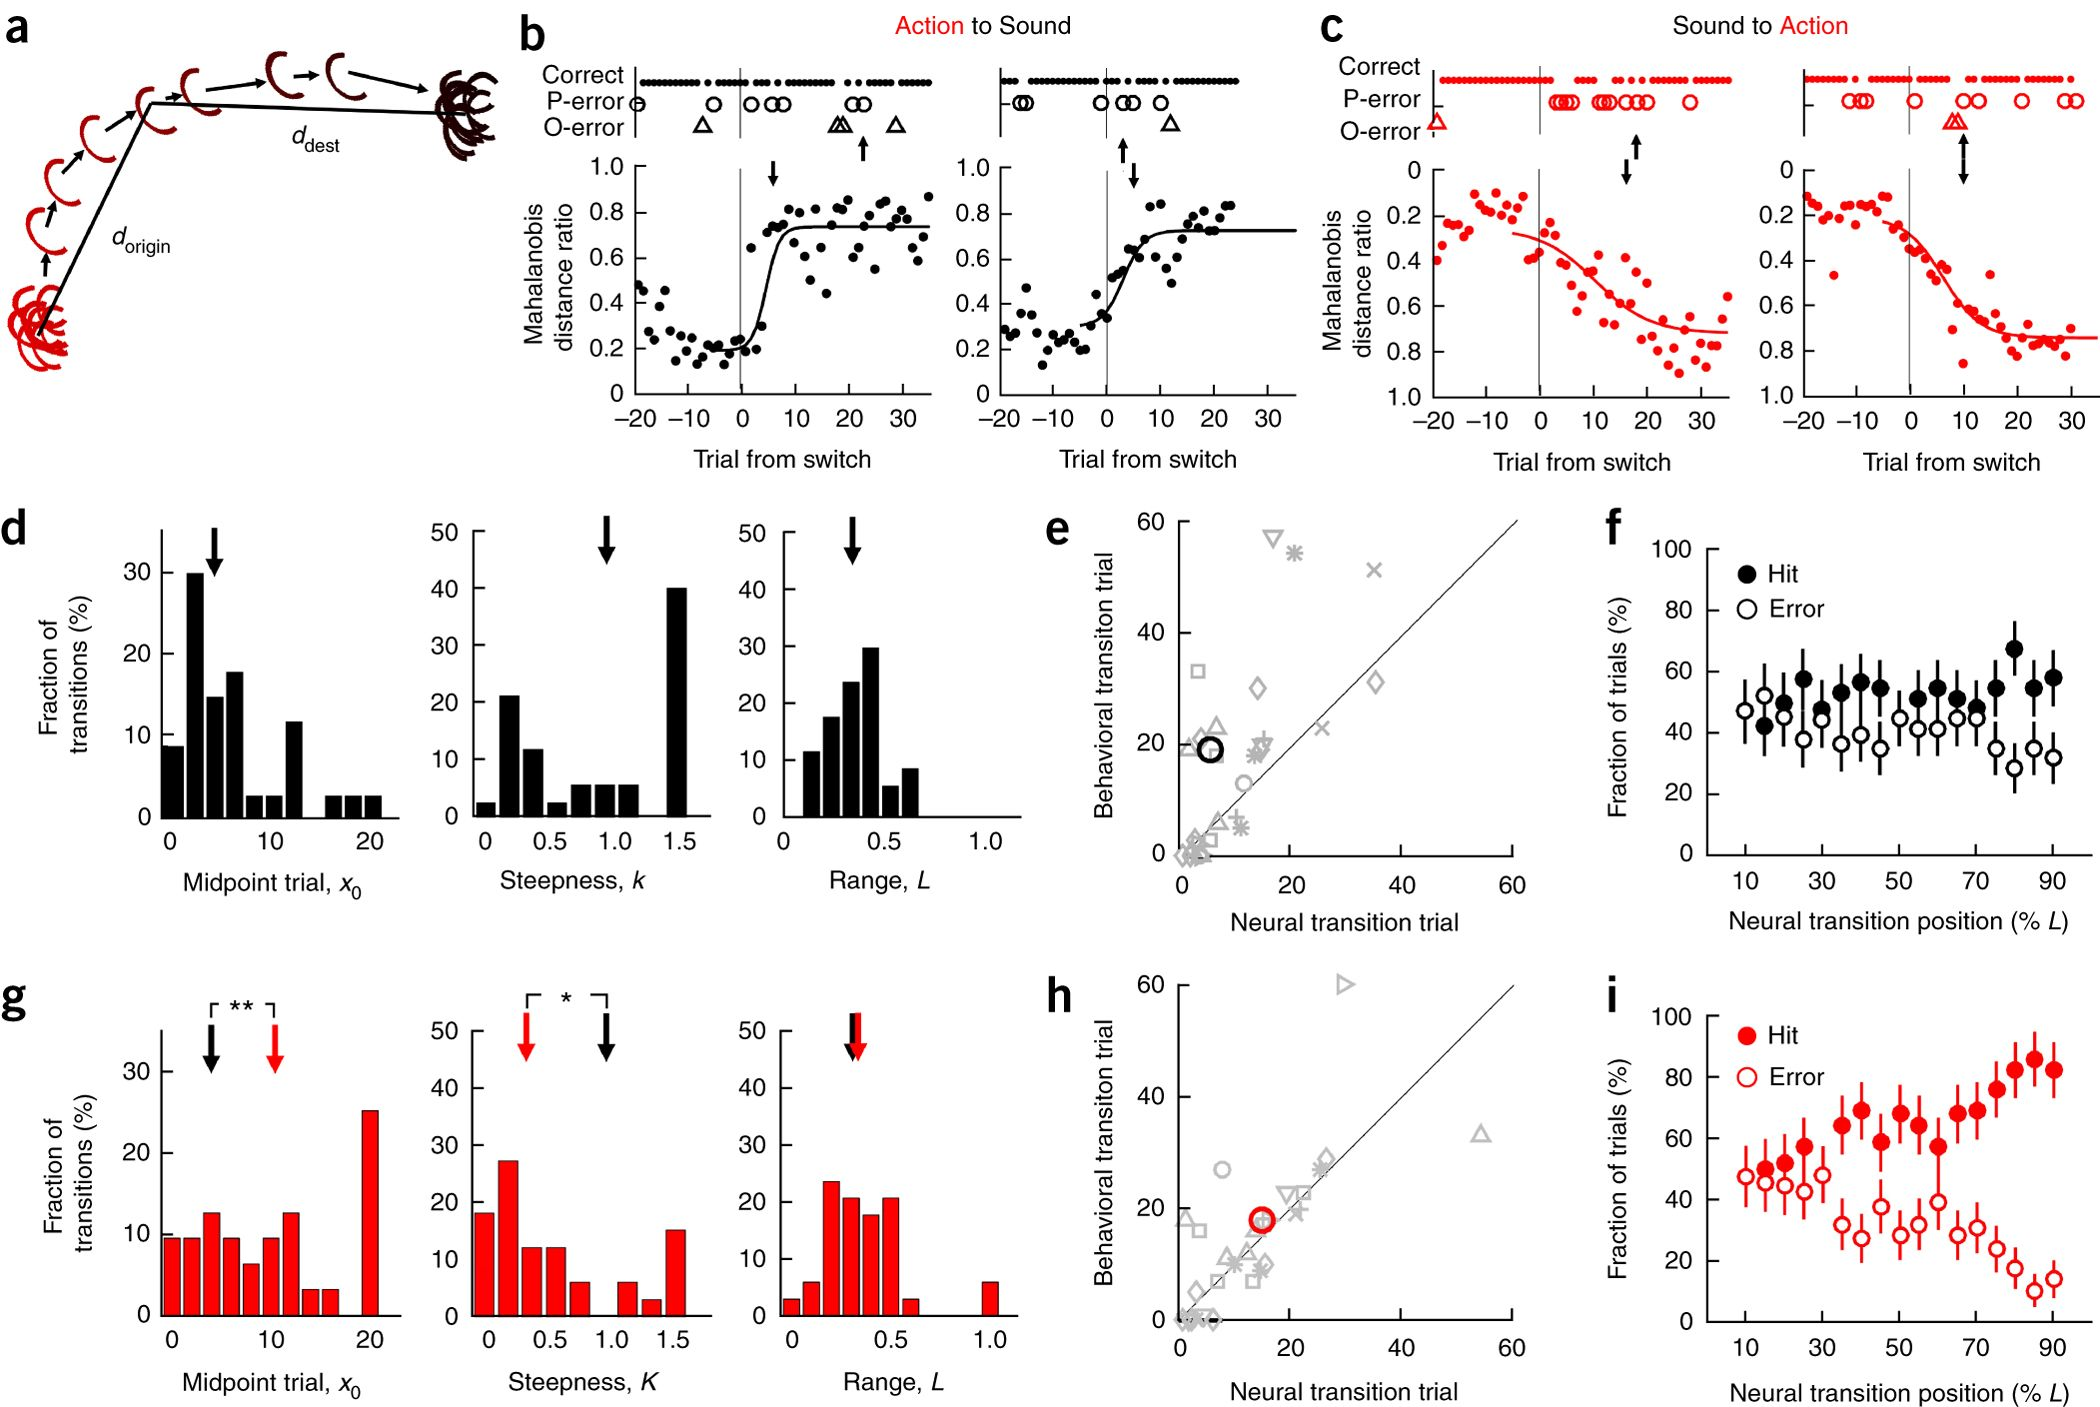
\includegraphics[width=\textwidth]{Figures/NN_fig4.jpg} 
\end{center}

\caption[Transitions in ensemble activity occur earlier and more abruptly following switch to sound rule]
{Caption}

\label{fig:NN_fig4}
\end{figure}

Comparisons of the transition dynamics following a switch into conditional versus unconditional rules uncovered marked differences. Out of 33 action-to-sound and 38 sound-to-action transitions, 33 and 35 switches, respectively, could be fit with a logistic function to compare the onset and rate of shifts in population activity patterns (Fig. 4b,c). State transitions associated with the shift to sound-guided responses occurred after only several trials, much earlier than with shifts into repeated actions (REF Fig. 4d,g; sound: midpoint trial, $x_0 = 4.0$, action: $x_0 = 10.4$, median; $p = 0.007$, $z = 2.70$, Wilcoxon rank-sum test). Furthermore, breaking from repetitive to sound-guided responding involved transitions that were more abrupt (sound: steepness, $k = 1.02$, action: $k = 0.35$, median; $p = 0.03$, $z = -2.17$, Wilcoxon rank-sum test). These differences in neural dynamics were not due to behavioral differences, because in this set of experiments trials to criterion were similar for the two rule types (sound: 39, action: 38, median; $p = 0.9$, $z = 0.09$, Wilcoxon rank-sum test; REF Supplementary Fig. 1a). 

Overall, these results suggest that ensemble activity patterns in M2 shift earlier and more steeply when animals are required to abort repetitive actions and engage conditional associations to perform sound-guided behavior.

To what extent must population activity resemble the final ensemble state in order to improve behavior? To address this question, we performed two analyses to compare the timing of neural and behavioral transitions. In the first analysis, we defined `transition trials' for behavior (trials to criterion minus 20, the sliding window for assessing criterion) and neural ensemble activity (Mahalanobis distance ratio equaling 75\% L based on logistic fit; see Methods). Block-by-block paired comparisons of neural and behavioral transition trials showed that ensemble activity in M2 shifted before the recovery of behavioral performance when adapting to conditional rules (Fig. 4e and Supplementary Fig. 6; $p = 0.003$, $z = -2.96$; Wilcoxon signed-rank test). By contrast, neural and behavioral changes occurred at around the same time for shifts to unconditional responding (Fig. 4h; $p = 0.19$, $z = 1.32$; Wilcoxon signed-rank test). 

We should note, however, that the definitions used for transition trials were arbitrary. Therefore, we performed a second, less biased analysis in which we determined the mean performance at the behavioral trial corresponding to a series of different neural transition locations. Compared with shifts to action trials (Fig. 4i), transitions to sound-guided trials were associated with hit and error rates that diverged later (Fig. 4f), indicating that behavioral improvement occurred later along the time course of neural transitions. 

Taken together, results of these two analyses suggest that when shifting to sound-guided actions, neural ensemble transitions in M2 are nearly complete before behavioral performance improvement can be detected.

\nnsub{Distinct Activity Patterns Accompany Rule Implementations}
Our results indicated that rule shifts are associated with distinct transitions in network activity. This leads naturally to the question of what ensemble dynamics accompany successful rule implementation. We examined trajectories associated with correct responses in the 20 trials before the switch, when response strategies had stabilized ($\ge 85\%$ correct by task design). 

Figure 5a shows the trajectories of a 56-cell ensemble for left and right responses during sound-guided trials. The trajectories were initially indistinguishable and then diverged sharply after the animal made a response. Expanding this analysis to include action blocks revealed population activity patterns that occupied additional, distinct subspaces within the same representational space (Fig. 5b).
\begin{figure}[htbp]

\begin{center}
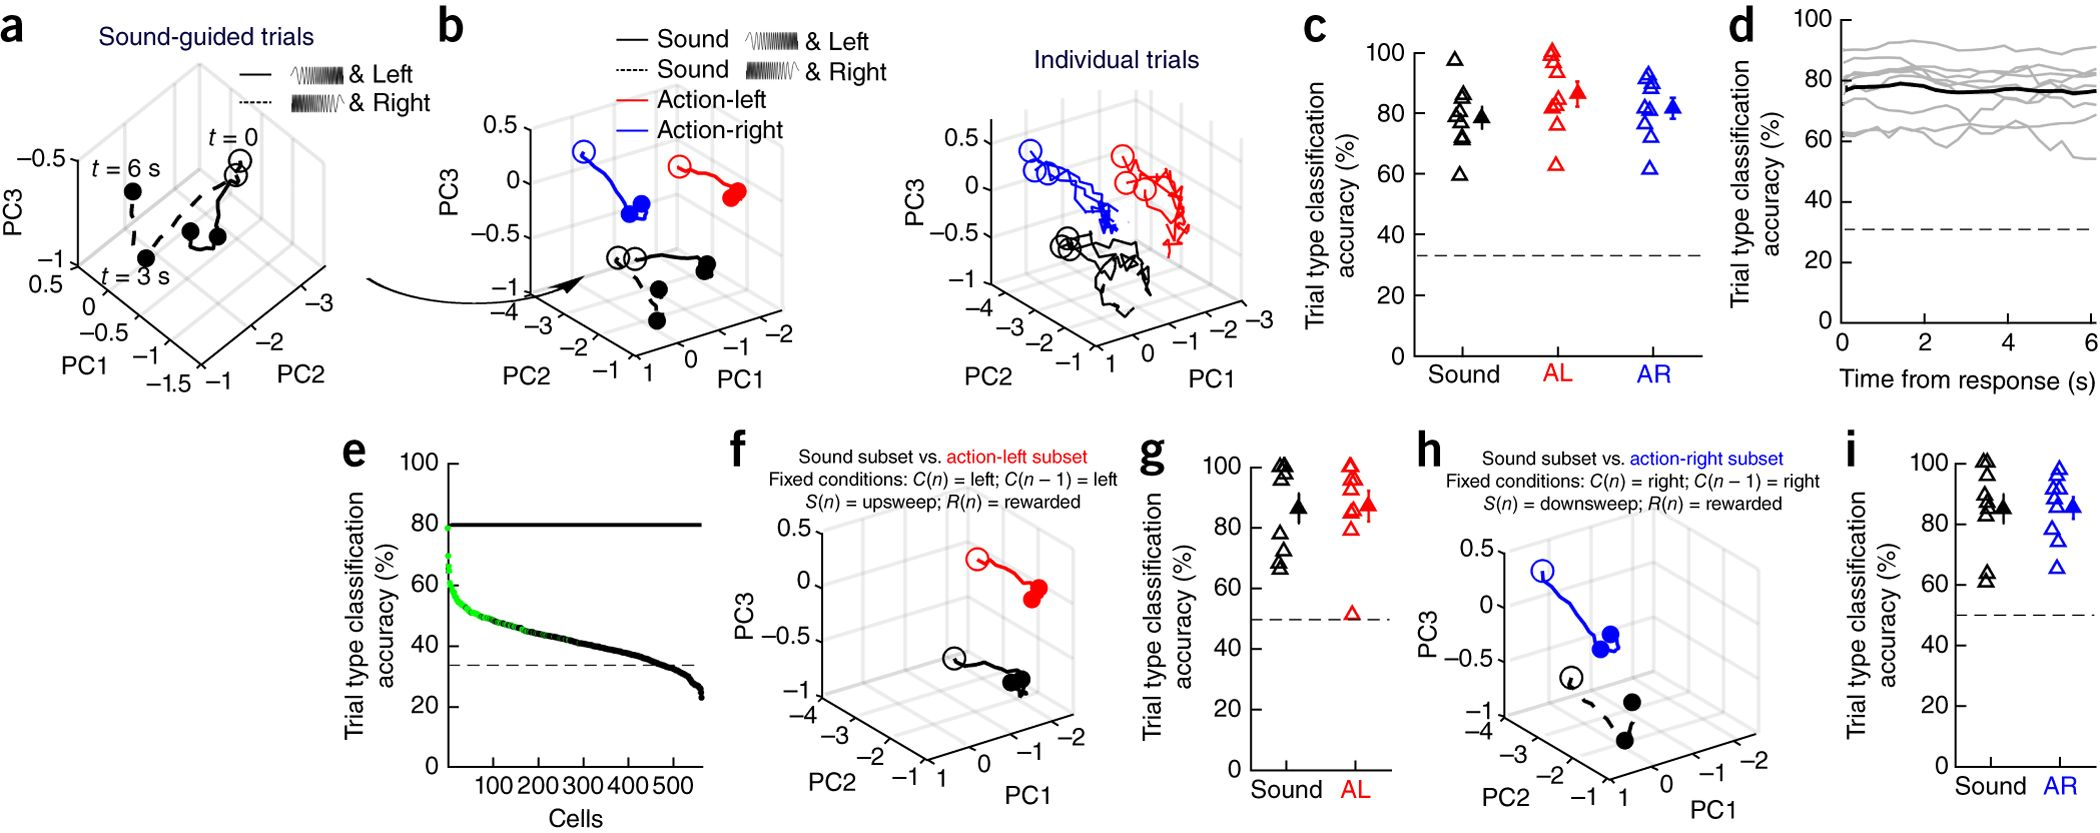
\includegraphics[width=\textwidth]{Figures/NN_fig5.jpg} 
\end{center}

\caption[Rule implementations are associated with distinct population activity patterns]
{Caption}

\label{fig:NN_fig5}
\end{figure}

To quantify rule representations present in the population code, we asked how accurately block type could be predicted from individual population activity vectors. For each session, we constructed a classifier based on linear discriminant analysis (see Methods). Testing each classifier with five-fold cross-validation revealed that in all cases trial type could be decoded well above chance (Fig. 5c; sound: $78 \pm 3\%$, action-left: $86 \pm 4\%$, action-right: $82 \pm 3\%$; versus chance level of 33\%, $p = 1 \times 10^{-6}$, $1 \times 10^{-6}$, $5 \times 10^{-7}$; $t(8) = $ 13.2, 12.8, 14.3; one-sample t-test; $N = 9$ sessions). 

Repetition of this analysis using a moving window yielded high decoding accuracy at all times during a trial (Fig. 5d), consistent with a global shift in engagement of the network rather than a simple change in the processing of cue, action or outcome related signals. 

Next we asked whether accuracy of the ensemble classifier could have been driven by a few highly rule-selective cells. When classifiers were trained on $\Delta F/F$ of individual cells, we found that 27\% of the cells could be used to decode block types at rates above chance; however, accuracy fell along a continuum and at levels below the accuracy of the ensemble (Fig. 5e). 

To ensure that the differences in trajectories and decoding accuracies were not due to simple sensory or motor parameters, we computed trajectories with matched stimulus, prior choice, current choice and outcome conditions. Analyses of these congruent trials, which differed only by rule, yielded similar results (Fig. 5f–i and Supplementary Fig. 7a–d). 

Taken together, these results indicate that the behavioral implementation of specific conditional and unconditional rules is associated with distinct network activity patterns in M2, such that population activity from any time during behavior can be used to decode task contingencies with high accuracy.

\nnsub{Activity Toggles between Rule-Related Patterns}
When animals solve trials with the same contingencies a second time, do M2 ensembles revisit similar activity patterns or does population activity migrate to a previously uncharted region of state space? Our task was well suited to address this question because blocks of the same trial type were presented multiple times within the same behavioral session. 

Figure 6a shows an example set of neural circuit trajectories for the first 12 trial blocks within one behavioral session, in which trajectories could be clearly grouped by block type and not by their temporal order. 
\begin{figure}[htbp]

\begin{center}
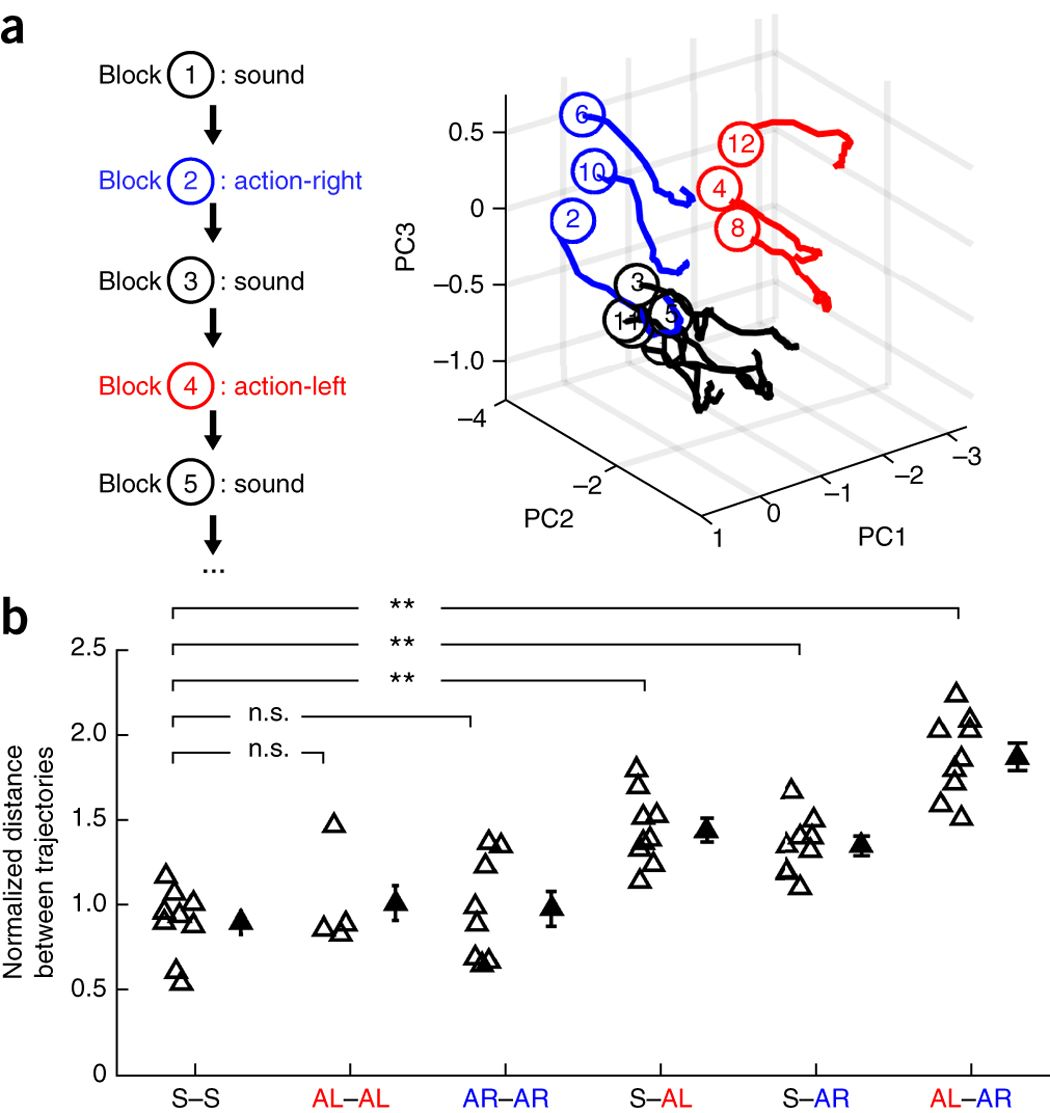
\includegraphics[width=\textwidth]{Figures/NN_fig6.jpg} 
\end{center}

\caption[M2 ensembles revisit previous activity patterns upon re-exposure to corresponding rule]
{Caption}

\label{fig:NN_fig6}
\end{figure}

To quantify the representational similarity of ensemble dynamics on a block-by-block basis, we calculated the mean Euclidean distances between all possible pairwise comparisons of trajectories within an experiment (see Methods). We found that neural circuit trajectories from blocks of the same type had a relatively small distance of separation and were similarly compact (Fig. 6b and Supplementary Fig. 7e,f; for sound (S), action-left (AL) and action-right (AR): S–S versus AL–AL: $p = 0.6$, $W = 3$; S–S versus AR–AR, $p = 0.5$, $W = 13$; Wilcoxon signed-rank test). By contrast, trajectories from different block types were represented by markedly different ensemble activity (S–S versus S–AL, $p = 0.004$, $W = 0$; S–S versus S–AR, $p = 0.004$, $W = 0$; S–S versus AL–AR, $p = 0.004$, $W = 0$; corrected $\alpha = 0.01$, Wilcoxon signed-rank test with Bonferroni correction). 

These results indicate that, during adaptive decision-making, M2 toggles between distinct functional configurations as the animal repeatedly engages corresponding changes in task demands.

\nnsub{Comparison of Task-Related Neural Dynamics in M2, ALM and V1}
Next, we sought to determine whether the observed neural dynamics are specific to M2 or may also be found in other brain regions. For this purpose, we imaged neural ensembles in layer 2/3 of anterior lateral motor cortex (ALM; $65 \pm 6$ cells per field of view, $mean \pm SEM$; $N = 8$ sessions from 4 mice; Supplementary Fig. 1b) and primary visual cortex (V1; $57 \pm 7$ cells per field of view; $N = 4$ sessions from 2 mice; Supplementary Fig. 1c) to compare with the data from M2 ($62 \pm 6$ cells per field of view; $N = 9$ sessions from 5 mice). ALM has been implicated in motor planning and execution37,38; however, it is $\sim 1.5$ mm distant from M2, and the relationship between the two frontal cortical regions is not understood. V1 was chosen as a control region because the task was performed in the dark and involved no visual stimulus. 

Multiple linear regression analysis showed that M2 neurons robustly encoded not only the choice of the current trial, but also the choices of the two prior trials (Fig. 7a). A higher proportion of cells in ALM encoded the current choice; however, the signals decayed faster, resulting in weaker encoding of prior choices (Fig. 7b). Activity of M2 and ALM neurons could prefer either the ipsilateral or contralateral direction (Supplementary Fig. 8a,b), consistent with prior studies30,38. Unexpectedly, choice signals were also observed in V1 (Fig. 7c). Choice selectivity in V1 was relatively weak, and $\Delta F/F$ was almost always higher when animals made an ipsilateral choice (REF Supplementary Fig. 8c). Because choice signals in V1 were transient and animals performed the task in the dark, we conjecture that the selectivity might relate to corollary discharge. 

To investigate ensemble activity, we employed the same dPCA and linear classifier analyses used for M2. We found that rule type could be decoded with high accuracy using ensemble activity from ALM (matched sound, action-left trials: $78 \pm 4\%$, $t(7) = 6.94$; $p = 2 \times 10^{-4}$; matched sound, action-right trials: $78 \pm 3\%$, $t(7) = 8.68$; $p = 5 \times 10^{-5}$; versus chance level of 50\%, one-sample t-test; REF Fig. 7d), but at a much worse rate for V1 (matched sound, action-left trials: $58 \pm 5\%$, $t(3) = 1.88$; $p = 0.2$; matched sound, action-right trials: $67 \pm 4\%$, $t(3) = 3.76$; $p = 0.03$). Therefore, both ALM and M2 exhibited task-specific ensemble activity patterns. 

However, unlike what we found in M2, characterization of ensemble transitions in ALM did not reveal significant differences between switches to sound versus action blocks (sound: $x_0 = 8.2$, action: $x_0 = 10.2$, median; $z = 1.62$, $p = 0.11$; sound: $k = 0.37$, action: $k = 0.56$, median; $z = 0.89$, $p = 0.4$; Wilcoxon rank-sum test; REF Fig. 7e). There were also no detectable timing differences between neural and behavioral transitions in ALM (sound: $p = 0.5$, $z = 0.61$; action: $p = 0.13$, $z = -1.50$; Wilcoxon signed-rank test; neural transition defined as 75\% L). 

Taken together, these data indicate regionally specific ensemble dynamics associated with adaptive behavior.

% Discussion
\section{Discussion}

The results of our study support two novel insights regarding the function of higher-order motor cortex in adaptive choice behavior. Firstly, fast and slow ensemble transitions are neural signatures for distinct phases of voluntary behavior. A comparison between transitions was possible because our task design allowed for multiple shifts between multiple contingencies within a single behavioral session. Secondly, the relative timing of neural and behavioral shifts, as well as the specific deficits following inactivation, highlighted a leading role for this region in the engagement of sensory cue-guided actions (Fig. \ref{fig:NN_figS9}). 

\input{Figures/NN_FigS9.tex}

This conclusion contrasts with previous studies of homologous or nearby prefrontal cortical regions, in which neural changes closely match or lag the time course of behavioral adaptation \citep{mitz1991learning,pasupathy2005different,durstewitz2010abrupt}. One explanation may be that prior studies have focused on the learning of novel sensorimotor mappings or new rules, whereas our task required animals to repeatedly disengage and re-engage the learned associations needed in sound-guided trials. 

Although this task shares important features with other assays for flexibility, there are also crucial differences. In contrast to paradigms that use a contextual cue to instruct rapid executive control on a trial-by-trial basis \citep{mante2013context,stokes2013dynamic,duan2015requirement}, animals in our experiment adapted on a time scale of tens of trials (Fig. 1c). This relatively slow rate of adaptation resembles that of learning during arbitrary visuomotor mapping, where the animal's basis for action selection is updated gradually based on reward feedback \citep{pasupathy2005different,asaad1998neural}. 

Our task also differs from other strategy- or set-shifting tasks for rodents \citep{durstewitz2010abrupt,darrah2008interaction}, in the sense that we used nonspatial stimuli that do not conform to classical definitions of exemplars or sets. Instead, the paradigm we used consisted of blocks of trials that required the subject to shift between conditional and non-conditional approaches to action selection. 

Analysis of the types of errors made during training suggests that mice perform two-choice auditory discrimination in part by suppressing a prepotent tendency to repeat a rewarded choice. Action trials could thus be considered a natural strategy to the animal, whereas sound-guided trials require weeks of training to achieve high performance. One caveat for our task is that animals are likely to have different degrees of learned and intrinsic familiarity for sound versus action trials. In principle, mice may solve the task by ignoring sensory information completely during action blocks. However, the temporally structured lick rates during action blocks (Fig. 1e) strongly suggest use of the stimulus for gating lick responses. 

We found that bilateral inactivation of M2 selectively impaired the shift into sound-guided actions. This observation is highly consistent with results of dorsal premotor lesions in primates, which disrupt both the learning of novel visuomotor associations and the engagement of previously learned mappings \citep{petrides1985deficits,halsband1985premotor,nixon2004cortico}. Adaptation to action blocks was facilitated by M2 inactivation. This effect could result from a tendency to repeat the prior choice \citep{sul2011role}: if M2 normally biases animals toward sensory-cue-guided actions, then inactivation may remove an important brake on the unconditional strategy. In our experiments, M2 inactivation slowed but did not preclude the eventual transition to high performance on sound-guided trials. This suggests that, at least for trained mice, two-choice auditory discrimination alone does not require M2 and may be subserved by other circuits \citep{znamenskiy2013corticostriatal}. Furthermore, we take the opposing effects of inactivation on shifts to sound-guided versus repeated actions as evidence that mice perform the task by balancing the use of conditional and unconditional responses.

A key finding of this study concerns how specific parameters of ensemble activity transitions may relate to behavior. We found that ensemble transitions were more abrupt when animals needed to retrieve and begin using conditional associations. These fast transitions may be related to those observed in medial prefrontal cortex, which have been interpreted as neural correlates of insight \citep{durstewitz2010abrupt} or as the abandonment of an inadequate internal model at the onset of exploration \citep{karlsson2012network}. 

On what quantitative basis should transitions be classified as abrupt or gradual? We compared the steepness of these transitions directly to the slower transitions that accompanied adaptation to action blocks. Moreover, ensemble transitions occurred after only a few errors, whereas behavioral improvements took tens of sound-guided trials (Fig. 4e,f). The difference in neural and behavioral timing suggests that M2 neural activity had mostly adjusted while the animal was still systematically responding in an unconditional manner. M2 may facilitate the engagement of sound-guided behavior by biasing the use of sensory information, suppressing repetitive actions, or both. By contrast, prior studies show that when an animal must acquire novel arbitrary associations, changes in cortical activity track behavioral improvements \citep{mitz1991learning,brasted2004comparison} and lag the more rapid remapping in the striatum \citep{pasupathy2005different}. A major difference between these studies of fast learning and our study is that the auditory–motor associations were already well learned in our task.

We found that multiple rules were each associated with a distinct subset of population activity patterns. Such task-dependent changes in neural activity are reported in multiple frontal cortical regions across species \citep{asaad2000task,rich2009rat,rodgers2014neural,durstewitz2010abrupt,wallis2001single}. By asking the animal to shift repeatedly during a single session, we found that the network could return to a previously employed functional configuration to meet similar behavioral demands. This back-and-forth toggling of ensemble activity is reminiscent of the ensemble remapping observed in CA1 of the hippocampus during repeated exposure to spatial contexts \citep{wills2005attractor,leutgeb2005independent}. One study reported that changes in environmental context also cause network activity shifts in the rodent medial prefrontal cortex. However, the ensemble code was not identical upon re-exposure, potentially owing to a systematic drift over time \citep{hyman2012contextual}. The divergent findings of repeatable versus drifting network states in the rodent frontal cortex could reflect regional differences or differences in how frontal areas encode cognitive versus environmental variables.

Several lines of evidence support the idea that the neural dynamics in M2 reflect changes in internal processes (for example, representation of task contingencies or motor planning and preparation) rather than differences in overt physical movements. Firstly, three different ensemble analyses with matched, congruent trial conditions indicated distinct neural dynamics in sound and action blocks (Fig. 5f–i and Supplementary Fig. 7), despite a lack of observable difference in motor output for the same sets of trials (Fig. 1e and Supplementary Fig. 2). Secondly, neural signals related to motor execution should be strongest at the time of response. Instead, we found that the rule-specific separation of population activity patterns was substantially above chance at all times across a trial (Fig. 5d). Perhaps the strongest evidence is that muscimol inactivation of M2 had no detectable effect on motor output (Supplementary Fig. 5), while clearly affecting behavioral flexibility.

What is the purpose of functional reconfiguration during adaptive decision-making? Ensemble activity patterns within multiple network subspaces reflect the diversity of neural representations in M2. Recent studies indicate functional roles for long-range projections from rodent M2 to sensory cortices \citep{schneider2014synaptic,manita2015top} and dorsal striatum \citep{rothwell2015input}. Appropriate shifts in neural representations could allow M2 to exert differential top-down control in a task-dependent manner. Further study regarding the downstream impacts of frontal network transitions may yield insights into neuropsychiatric disorders in which cognitive flexibility is impaired. Plausibly, the cognitive rigidity characteristic of disorders such as schizophrenia could result from an inability of frontal cortical networks to shift or maintain stable ensemble states.

% Materials & Methods
%\newpage
\section{Materials \& Methods}

\subsection*{Animals}
We used adult male mice with C57BL/6J genetic background. Mice were housed in groups of 3--5, in 12-h/12-h light-dark cycle (lights off at 19:00), and most experiments were performed in late afternoons and evenings (16:00--midnight). At the start of experiments, mice were P51--117. No statistical tests were used to predetermine sample sizes, but sample sizes for this study are similar to those generally employed in the field. All experimental procedures were approved by the Institutional Animal Care and Use Committee, Yale University.

\subsection*{Surgery}
Mice underwent two surgeries. For each surgery, the mouse was anesthetized with 2\% isoflurane in oxygen during induction, which was then lowered to 1–1.5\% for the remainder of the surgery. The mouse was placed over a water-circulating heating pad (TP-700, Gaymar Stryker) in a stereotaxic frame (David Kopf Instruments). Before the operation, the mouse was injected with carprofen (5 mg/kg, s.c.; \#024751, Butler Animal Health) and dexamethasone (3 mg/kg, s.c.; Dexaject SP, \#002459, Henry Schein Animal Health). The mouse was injected with carprofen immediately after surgery (5 mg/kg, s.c.) and each day for the following 3 d (5 mg/kg, s.c.). 

For the first surgery, an incision was made to expose the skull. Based on stereotaxic coordinates, the center location of the mouse secondary motor cortex (M2; AP 1.5 mm and ML $-0.5$ mm relative to bregma) was marked over the right hemisphere. In other experiments, we targeted the anterior-lateral motor cortex (ALM; AP 2.5 mm, ML $-1.5$ mm) or the primary visual cortex (V1; AP $-3.8$ mm, ML 2.0 mm) in the right hemisphere. A stainless steel head plate (eMachineshop) was affixed to the skull with Metabond (C\&B, Parkell, Inc.), and a thin layer of clear Metabond was then applied to cover the entire skull. Mice were given at least 1 week to recover before behavioral training (see below). 

Once mice reached a performance criterion of $>90\%$ correct rate on three consecutive days and was ready for imaging experiments, a second surgery was performed under anesthesia. Using a dental drill, a 3-mm-diameter craniotomy was made at the target location, which had been marked previously and remained visible through the Metabond. Dura was left intact and was irrigated with artificial cerebrospinal fluid (aCSF, in mM: 5 KCl, 5 HEPES, 135 NaCl, 1 MgCl2, 1.8 CaCl2; pH 7.3). 

Using a glass micropipette attached to a microinjection system (Nanoject II, Drummond), 32--46 nL of AAV1-Syn-GCaMP6s-WPRE-SV40 ($5 \times 10^{13}$ titer; UPenn Vector Core) was injected at a depth of 400 \unit{\micro\meter} below dura at each of four locations: the vertices of a square 200 \unit{\micro\meter} wide, centered on the target coordinates. The glass micropipette was left in place for 5 min after injection to reduce backflow. A drop of warmed agarose solution (1.2\% in ACSF, Type III-A, High EEO, A9793, Sigma-Aldrich) was then applied to the cortical surface. 

A two-layer glass window was fabricated by first etching out a 2-mm-diameter circle from \#0 thickness glass cover slip, then bonding with UV-activated polymer (61, Norland Optical Adhesive) to a \#1 thickness, 3-mm-diameter round glass cover slip (64-0720 CS-3R, Warner Instruments). This glass window was then placed against the cortical surface. While applying light pressure, cyanoacrylate glue was added to the rim to attach the glass to the skull and Metabond. Mice were again given at least 1 week to recover before resuming behavioral training. Imaging experiments began when behavioral performance criterion was reached. 

Eight of 11 mice went through this procedure involving two surgeries. For the remaining three mice, the head plate implant, viral injection and window implant procedures were performed in the same surgery before behavioral training.

\subsection*{Behavioral Setup}
For head-fixed mouse behavior, we used a training apparatus with two lick ports, thus enabling two alternative choices \citep{guo2014flow}. Two metal screws were used to affix the head plate of the mouse onto a stainless steel mount. The mouse was then restrained inside an acrylic tube, which restricted gross body movements but allowed postural adjustments. 

The lick ports were fabricated from stainless steel 20-gauge needles, which were positioned at $90 \degree$ and $270 \degree$ with respect to the mouse's head orientation, and held in place by a 3D-printed plastic part mounted on a micromanipulator for fine positional adjustment. Water was delivered at the ports by gravity feed and the liquid volume was controlled by pneumatic valves (EV-2-24, Clippard) calibrated with an intravenous dripper to deliver $\sim 2$ \unit{\micro\liter} per pulse. A battery-operated touch detector circuit signaled when the mouse's tongue contacted a lick port. 

Auditory stimuli were played through computer speakers placed directly in front of the animal. The intensity of the auditory stimuli was calibrated to $\sim 85$ dB peak amplitude. 

Water delivery, lick detection and sound presentation were connected to a desktop computer via a data acquisition board (USB-201, Measurement Computing). Presentation software (Neurobehavioral Systems) controlled the entire behavioral system.

Behavioral training was performed inside the closed compartment of an audio-visual cart that was dark and soundproofed with acoustic foam (5692T49, McMaster-Carr). An infrared webcam was used to monitor the animal while in the rig. For imaging, mice were tested using a replica of the behavioral training setup under a two-photon microscope.

\subsection*{Adaptive Decision-Making Task}
To motivate participation in the task, water consumption was restricted to behavioral sessions. Mice were trained for 1 session per day, 6 d per week. On the non-training day, water was provided \textit{ad libitum} in the home cage for 15 min. 

The mice were trained through four phases to shape their behavior. Phase one ($\sim 2$ d): mice were habituated to head fixation in the behavior box and trained to lick either one of the two ports for water reward. Mice were advanced to the next phase when they made $>100$ responses in a session. 

Phase two ($\sim 2$ d): mice were trained to sample both ports. Here mice were required to lick the left port to obtain water rewards three times, followed by the right port for the next three rewards, and so on. Mice were advanced to the next phase when they made $> 100$ correct responses in a session. 

Phase three ($>15$ d): animals underwent training for two-choice auditory discrimination. One of two auditory cues was presented to begin each trial---a 2-s-long train of 0.5-s-long logarithmic frequency modulated sweeps from 5 to 15 kHz (`upsweep') or from 15 to 5 kHz (`downsweep'). These stimuli were interleaved randomly from trial to trial. At 0.5 s following the onset of the auditory cue, a response window opened, lasting for a duration of 1.5 s. The first lick within this response window was registered as its response for the trial. All other licks were logged but had no consequences. Once a response was recorded, playback of the auditory cue was terminated. 

A correct response, i.e., a left lick for upsweep or a right lick for downsweep, resulted in immediate delivery of 2 \unit{\micro\liter} of water from the corresponding port. The next trial would begin 7 s following response. Incorrect responses resulted in 2 s of white noise presentation, with the next trial beginning 5 s later. Thus, each trial had a total duration within a range from 7.5 to 9 s. Animals were allowed to perform trials until satiated (20 consecutive misses), typically after $\sim 60$ min. 

Training continued daily until a correct rate of $>90\%$ was attained for 3 consecutive days. For imaging experiments, mice were then trained under the two-photon microscope (with laser turned off) for habituation to the recording setup. All mice were able to discriminate at $>90\%$ correct rate after 1--3 d of re-training. 

Finally, mice were tested on the adaptive decision-making task. The task always began with a sound block (S) indistinguishable from the two-choice auditory discrimination task. However, once the mouse reached a performance criterion of $>85\%$ correct for the last 20 trials, the stimulus–response-outcome contingencies changed from being sound- to action-guided. In action-guided trials, task structure was identical to sound-guided trials. However, the correct response became fixed to one response direction, for example, always left, regardless of the stimulus identity. No cue signaled the change in contingencies. 

When the mouse reached performance criterion again, another block switch occurred. A sound block was always followed by an action block and vice versa. The second block was randomly chosen for each experiment to be action-left (AL) or action-right (AR). However, once the first action block was chosen, the block sequence became fixed for the remainder of the session. Therefore, the sequence of blocks could be one of two possibilities: (S-AL-S-AR-S- \ldots) or (S-AR-S-AL-S \ldots). 

Each session was terminated after 20 consecutive misses (trials with no response). Mice typically performed the adaptive decision-making task for 60--90 min. Following each adaptive decision-making test, mice resumed daily two-choice auditory discrimination until the next recording session, up to a maximum of 7 adaptive decision-making tests.

\subsection*{Two-Photon Calcium Imaging}
The two-photon microscope (Movable Objective Microscope, Sutter Instrument) was controlled using ScanImage software51. The excitation source was a Ti:Sapphire femtosecond laser (Chameleon Ultra II, Coherent). Excitation intensity was controlled by a Pockels cell (350-80-LA-02, Conoptics) and focused onto the sample with a $20\times$, N.A. 0.95 water immersion objective (Olympus). The time-averaged excitation laser intensity was 90--100 mW after the objective. 

To image fluorescence transients from GCaMP6s-expressing neurons, excitation wavelength was set at 920 nm, and emission was collected from 475--550 nm with a GaAsP photomultiplier tube. Time-lapse images were acquired at a resolution of $256 \times 256$ pixels and a frame rate of 3.62 Hz using bidirectional scanning. To synchronize behavior with imaging, a TTL pulse was sent at the beginning of each trial from the data acquisition board of the behavioral system to the imaging system to act as an external trigger for initiating image acquisition.

\subsection*{Neural Inactivation}
Mice were implanted with a head plate. The locations of M2 were marked on both hemispheres (AP 1.5 mm, ML $-0.5$ mm), and then covered with a thin layer of clear Metabond. Mice were then trained as described above, in preparation for the adaptive decision-making test. 

On the first day of testing, craniotomies were performed at the marked locations. Using a glass micropipette attached to a microinjection system (Nanoject II, Drummond), aCSF, with or without muscimol (5 mM, 46 nL per hemisphere; cat. \#195336, MP Biomedical), was injected at a depth of 400 \unit{\micro\meter} into M2 of both hemispheres. Behavioral testing began 1--3 h following injection. 

The same mice were tested after saline and muscimol treatments on consecutive days in a counter-balanced design, with no blinding. The mice were randomized to receive either saline or muscimol first in an alternating manner depending on the order in which they reached the behavioral performance criterion. Twelve mice were allocated for this experiment; however, one was excluded due to equipment malfunction during testing.

\subsection*{Histology}
Following experiments, mice were transcardially perfused with chilled formaldehyde solution (4\% in phosphate-buffered saline). The brains were sectioned with a vibratome and imaged with an inverted wide-field fluorescence microscope.

\subsection*{Analysis of Behavioral Data}
Timestamps of stimulus presentation, licks and water delivery were logged in a text file by Presentation software (Neurobehavioral Systems, Inc.). Scripts were written in MATLAB to parse the log files. 

`Perseverative errors' were defined as incorrect responses that would have been correct according to the contingencies of the last block of trials. For example, during an action-left block, the stimulus–response pairings of upsweep–left lick and downsweep–left lick would be `correct'. Downsweep–right lick would be a perseverative error, because this stimulus–response pairing would have been correct in the preceding sound-guided block. The remaining possible stimulus–response pairing, upsweep–right lick, would be classified as an `other error'. 

The number of trials performed included all correct and error trials, but excluded `miss' trials where the mouse failed to lick within the response window. Miss trials typically occurred near the end of the session when the mouse was satiated. 

The number of trials to criterion was defined as the number of trials performed in a certain trial block before reaching a performance criterion of 85\% correct for the last 20 trials. Therefore, the minimum value of this quantity is 20. 

Mean trials to criterion for each session was calculated excluding the first sound block, because contingency switches had not yet begun. Mean blocks per 100 trials, mean perseverative errors per block and mean other errors per block were calculated excluding the last block (i.e., trials after the last block switch). We often compared conditions before and after block switches, which were defined as the 20 trials before or following a block switch. 

The first lick time was defined as the time of the first lick after sound onset for each trial, even if this occurred before the start of the response window. The first lick time is thus a sum of the reaction time and movement time. For this measurement, we excluded trials in which the mouse licked within 0.5 s before cue onset, in which case the first lick may represent the continuation of a spontaneous lick bout rather than a reaction to the stimulus.

\subsection*{Analysis of Imaging Data}
Time-lapse fluorescence images were first corrected for x–y motion using the TurboReg plug-in \citep{thevenaz1998pyramid} for ImageJ \citep{schneider2012nih}. 

We wrote a graphical user interface in MATLAB to select cell bodies as regions of interest (ROIs). Values of pixels within an ROI were averaged within each frame to yield the cellular fluorescence measurement $F_C(t)$. For each cell, we estimated the neuropil signal by approximating the ROI area as a circle to estimate a radius $r$ \citep{peron2015cellular}, then creating an annulus-shaped neuropil area with inner and outer radii of $2r$ and $3r$. This neuropil area excluded pixels if they were part of the ROI of another cell body. Values of pixels within the annulus-shaped neuropil area were averaged to generate $F_N(t)$. To subtract the neuropil signal, we calculated $F(t) = F_C(t) - \alpha F_N(t)$, where $\alpha$ is a correction factor ranging from 0.2 to 0.6. The value of $\alpha$ was calibrated for each experiment to avoid overcorrection, by making sure that $F(t) > 0$ for each cell. 

For each ROI, the fractional change in fluorescence, $\Delta F/F (t)$, was calculated as

\begin{equation*}
    \frac{\Delta F}{F}(t) = \frac{F(t)-F_0(t)}{F_0(t)}
\end{equation*}

\noindent where $F_0(t)$ is the baseline fluorescence as a function of time. 

To estimate baseline, we first obtained $F_{image}(t)$, the mean pixel intensity for the entire $256 \times 256$ pixel field of view as a function of time. $F_0(t)$ was then calculated as

\begin{equation*}
    F_0(t) = F^{*} \times \frac{F_{0,image}(t)}{F^*_{0,image}}
\end{equation*}

\noindent where $F_{0,image}(t)$ is the 10th percentile of $F_{image}(t)$ within a sliding window of 10 min duration. $F^*$ and $F^*_{0,image}$ are the 10th percentile of $F(t)$ and $F_{0,image}(t)$ within the first 10 min of the session, respectively. We verified that $F_{0,image}(t)/F^*_{0,image}$ does not vary with specific choices or rule blocks, and thus serves the purpose of compensating for slow, full-field signal drifts due to non-physiological sources. 

We repeated the ensemble analyses with two other methods for calculating baseline: firstly, estimating $F_0(t)$ using the 10th percentile of $F(t)$, on a per-cell basis, with a moving window of 10 min duration; and secondly, estimating $F_0(t)$ using the 10th percentile of $F(t)$ from the entire session, i.e., without a moving window. These different ways to estimate baseline led to qualitatively similar results for all the ensemble analyses.

\subsection*{Analysis of Task-Related Activity and Choice Encoding}
To calculate trial-averaged fluorescence transients, we created time bins that were 0.5 s wide and assigned each $\Delta F/F (t)$ value at a particular time $t$ to the corresponding time bin relative to the animal's response. The binned $\Delta F/F (t)$ values were averaged to obtain trial-averaged $\Delta F/F (t)$. To estimate the uncertainty of the trial-averaged $\Delta F/F (t)$, a bootstrap analysis was performed by drawing fluorescence transients per trial, with replacement, up to the same number used to construct the trial average. The median and 95\% confidence intervals of trial-averaged $\Delta F/F (t)$ were estimated from 1,000 iterations of this bootstrap analysis. 

To quantify choice encoding, we performed multiple linear regression analysis on the $\Delta F/F (t)$ of each cell using the following equation:

\begin{equation*}
\frac{\Delta F}{F}(t) = a_0 + a_1 C_{n} + a_2 C_{n-1} + a_3 C_{n} C_{n-1} + a_4 C_{n-2} + \epsilon(t),\\
\end{equation*}

\noindent where $C_n$ is the choice made in the current trial, $C_{n-1}$ is the choice from the prior trial, $C_{n-2}$ is the choice from two trials ago, $\epsilon (t)$ is the error term, and $a_0 \ldots a_n$ are the regression coefficients. Left choices were coded as 1 and right as $-1$. 

A cell was deemed to encode one of the choice parameters or their interaction if $P < 0.01$ for the corresponding regression coefficient. To avoid confounds from rule and reward signals, we analyzed only sound-guided trials in which the outcomes of the current trial and prior trial were both reward. We did not analyze action trials because parameters such as $C_n$ and $C_{n-1}$ were highly correlated by virtue of the task structure---thus breaking a primary assumption underlying this type of analysis.

\subsection*{Analysis of Neural Ensemble Trajectories}
For state-space analyses, we used demixed principal component analysis \citep{machens2010functional} (dPCA). To prepare the imaging data for dPCA, we aligned $\Delta F/F$ traces from the first six seconds of each trial following the response. This alignment produced an array with dimensions ($cells \times time \times trials$). We then averaged across four trial types: $C_n = 1$ for pre-switch sound trials; $C_n = -1$ for pre-switch sound trials; $C_n = 1$ for pre-switch action trials; and $C_n = -1$ for pre-switch action trials---in all cases using only rewarded trials. This trial-averaged array ($cells \times time \times 4$) was input into the dPCA algorithm to demix time- and task-dependent variances and obtain principal components (PCs). 

To calculate neuronal trajectories, single-trial or trial-averaged $\Delta F/F$ traces were projected onto the first three PCs. To characterize similarities between trajectories across blocks, we calculated the trajectory for each block using the trial-averaged fluorescence across the 20 trials prior to the rule switch. 

The similarity between a pair of trajectories was quantified by calculating the mean Euclidean distance between trajectories at matching time points in state space. For pooled comparisons across experiments, the Euclidean distances were normalized by the dispersion population vectors from the corresponding experiment, calculated as the root mean square of the distances between all population vectors and the centroid of the vectors. 

To quantify how neural ensemble trajectories evolved on a trial-to-trial basis, we used the Mahalanobis distance, which is a measure of distance between one point and another collection of points. We defined the origin and destination as the population activity from the 20 trials preceding the current rule switch and the next rule switch, respectively. We were interested in the relative separation between the origin, an individual trial that occurred in between, and the destination. Therefore, for each time point within a trial, we calculated Mahalanobis distances, $d_{origin}(t)$ and $d_{dest}(t)$, from the corresponding population activity vector (one three-dimensional value) to those of the origin and destination, respectively (20 three-dimensional values each, estimated as the median across time for each trial). For each individual trial $n$, $d_{origin}(n)$ and $d_{dest}(n)$ were then estimated as the median distances for the $\sim 30$ time points within a trial. 

The location of an individual trial relative to the origin and destination was estimated as the ratio of Mahalanobis distances, $d_{origin}(n)/(d_{origin}(n) + d_{dest}(n)$). To summarize the relationship between this distance ratio and the number of trials from the rule switch, we then fit a logistic function,

\begin{equation*}
f(x) = \frac{L}{1+e^{-k(x-x_0)}} + L_{min}
\end{equation*}

\noindent where $x_0$ is the midpoint trial, $k$ is the steepness, $L$ is the range, and $L_{min}$ is the minimum value. The parameter $L_{min}$ was not fitted, but rather was estimated for each transition by calculating the mean Mahalanobis distance ratio using the five trials prior to each rule switch. 

We fit every neural ensemble transition using this method, but excluded those in which the midpoint trial $x_0 < -5$ or $x_0 > 200$, indicating a poor fit. Based on this criterion, we excluded none (0/33) of the action-to-sound shifts and 8\% (3/38) of the sound-to-action shifts in our analysis of M2 neural ensembles. For analysis of the ALM data set, we excluded 8\% (2/26) of the action-to-sound shifts and 3\% (1/32) of the sound-to-action shifts. 

When comparing behavioral and neural transitions, we defined `behavioral transition trial' as the number of trials to criterion (85\% correct for 20 consecutive trials) minus 20, i.e. the first in a series of 20 trials preceding the rule switch. The `neural transition trial' was defined as the trial when the first term of the logistic fit reached a value of 75\% $L$. That is, the trial $x$ that satisfies this equation:

\begin{equation*}
0.75L = \frac{L}{1+e^{-k(x-x_0)}}
\end{equation*}

This definition was arbitrary because it was unknown how much the population activity pattern must resemble the final pre-switch ensemble state in order to qualify as a transition. Therefore, in another analysis we first fit each neural transition with the logistic function and identified the behavioral trial corresponding to each 5\% $L$ step of neural transition from 10 to 90\% $L$. We then calculated the mean hit and error rates at the corresponding behavioral trials. The analysis provided a second description of the relationship between behavioral performance and neural transition without explicitly defining a transition trial.

\subsection*{Decoding population activity}
To determine how accurately trial type could be predicted from the ensemble activity, we gathered imaging frames that occurred between 0 to 6 s from time of response out of the frame-by-frame imaging data (i.e., $\Delta F/F (t)$). We then projected these $\Delta F/F (t)$ values onto the PCs determined from dPCA to obtain population activity vectors. This procedure reduced the dimensionality of our data from ($frames \times cells$) to ($frames \times 3$). 

Population activity vectors in this analysis were sampled from the last 20 trials of completed sound, action-left, or action-right blocks, and restricted to rewarded trials. Other trial types were not considered for the decoding analysis. We trained classifiers on a randomly chosen fraction (80\%) of the population activity vectors. Classifiers were based on linear discriminant analysis, using Mahalanobis distances with stratified covariance estimates (the `classify' function in MATLAB with `Mahalanobis' option). We then tested the performance of each classifier on the remaining 20\% of the population activity vectors, comparing classification results with actual trial types. This five-fold cross-validation process was repeated 1,000 times to obtain a median estimate of classifier accuracy. 

%***Resume initial formatting here (paragraph breaks, etc.)***
To investigate decoding accuracy across time, the timing information of each population activity vector relative to the time of response in each trial was retained. We then ran a separate decoding analysis on the population activity vectors measured during each time period, using a non-overlapping sliding window with duration of 0.28 s and step size of 0.28 s. This window duration is the inverse of frame rate, which was 3.6 Hz. To decode from single-cell activity, $\Delta F/F (t)$ of each cell was used instead of population activity vectors as inputs to construct the classifier.

\subsection*{Statistics}
Statistical tests were performed in MATLAB and are indicated in the main text or figure legends. Unless otherwise noted, a Wilcoxon signed-rank test was used for all paired comparisons. For two-sample, unpaired comparisons, a Wilcoxon rank-sum test was used. Paired t-tests were used for bin-wise analysis of lick rates. For quantification of choice signals as a function of time, multiple linear regression was first performed as detailed above; a binomial test was then applied to the proportion of cells significantly encoding choice within each time-bin. For ensemble decoding analyses, mean classification accuracy was tested against chance level using a one-sample t-test. For t-tests, the sampling distribution of the mean was assumed to be normal, but this was not formally tested. All t-tests were two-tailed.

% Acknowledgements
\nnsec{Acknowledgments}

We thank Daeyeol Lee, Marina Picciotto, and Jane Taylor for discussions; and Caroline Posner and Rachel Hannibal for assistance with behavioral training. The contents of this chapter were modified from a previously published research article: 

\smallskip 
\begin{singlespace}
Siniscalchi MJ, Phoumthipphavong V, Ali F, Lozano M, Kwan AC. Fast and slow transitions in frontal ensemble activity during flexible sensorimotor behavior. Nature neuroscience. 2016 Sep;19(9):1234.
\end{singlespace}

\subsection*{Author Contributions}
M.J.S. and A.C.K. conceived the project. M.J.S. performed all experiments. V.P. assisted with mouse surgery and inactivation experiments. F.A. and M.L. assisted with behavioral training and histology. M.J.S. and A.C.K. analyzed the data and wrote the manuscript.

\subsection*{Funding}
This work was supported by National Institute of Aging center grant P50AG047270 (A.C.K.), National Institute of Mental Health grant R21MH110712 (A.C.K.), NAR\-SAD Young Investigator Award (A.C.K.), National Institutes of Health training grant T32NS041228 (M.J.S.), National Science Foundation Graduate Research Fellowship DGE-1122492 (M.J.S.), and a Brown-Coxe Postdoctoral Fellowship (F.A.).



% Supplementary Figures
% \renewcommand{\figurename}{Supplementary Figure}

\clearpage
\section{Supplementary Figures}

\input{Figures/NN_FigS1.tex}
\input{Figures/NN_FigS2.tex}
\input{Figures/NN_FigS3.tex}
\input{Figures/NN_FigS4.tex}
\input{Figures/NN_FigS5.tex}
\input{Figures/NN_FigS6.tex}
\input{Figures/NN_FigS7.tex}
\input{Figures/NN_FigS8.tex}
\input{Figures/NN_FigS9.tex}

\clearpage
